\hypertarget{sasha-2112}{%
\chapter*{Sasha — 2112}\label{sasha-2112}}

Pain woke Sasha. Pain and a rumbling, jittery sensation within her body.

The pain coursed through her limbs, seeming to originate from a wellspring at the base of her neck. She remembered a quickly building sense of vertigo, of the whole of her perception growing fuzzy around the edges, and then\ldots{}nothing.

And then this.

She levered her eyes open slowly, carefully, and was greeted by an extreme close-up view of a dandelion. A dandelion. More dandelions. Cartoonishly fat bumblebees — for what bumbler is not cartoonish? — coursed among them in lazy Lissajous curves. They all avoided her with the polite patience of bees of all ilk.

``The fuck.'' The half-formed phrase tumbled out from between what felt like half-formed lips.

She carefully picked herself up off the ground, off the field of endless dandelions. The pain coursing through her body was quickly explained as she turned around. It appeared that she had fallen from a tall barstool. There stood before her a row of them lined neatly before a bar. \emph{The} bar. The one so familiar from countless nights and weekends loitering in the Crown Pub.

The bar stood alone in the field. No backing wall full of racks of bottles. No walls at all: beyond the bar was more endless field. No floor: the stools sprouted as easily from soil and grass as did the dandelions.

Dandelions.

That warm smell of fresh-baked muffins hung thick in the air. The warm air. The warm sun. The warm sky. The warm earth.

\AddToHookNext{shipout/after}{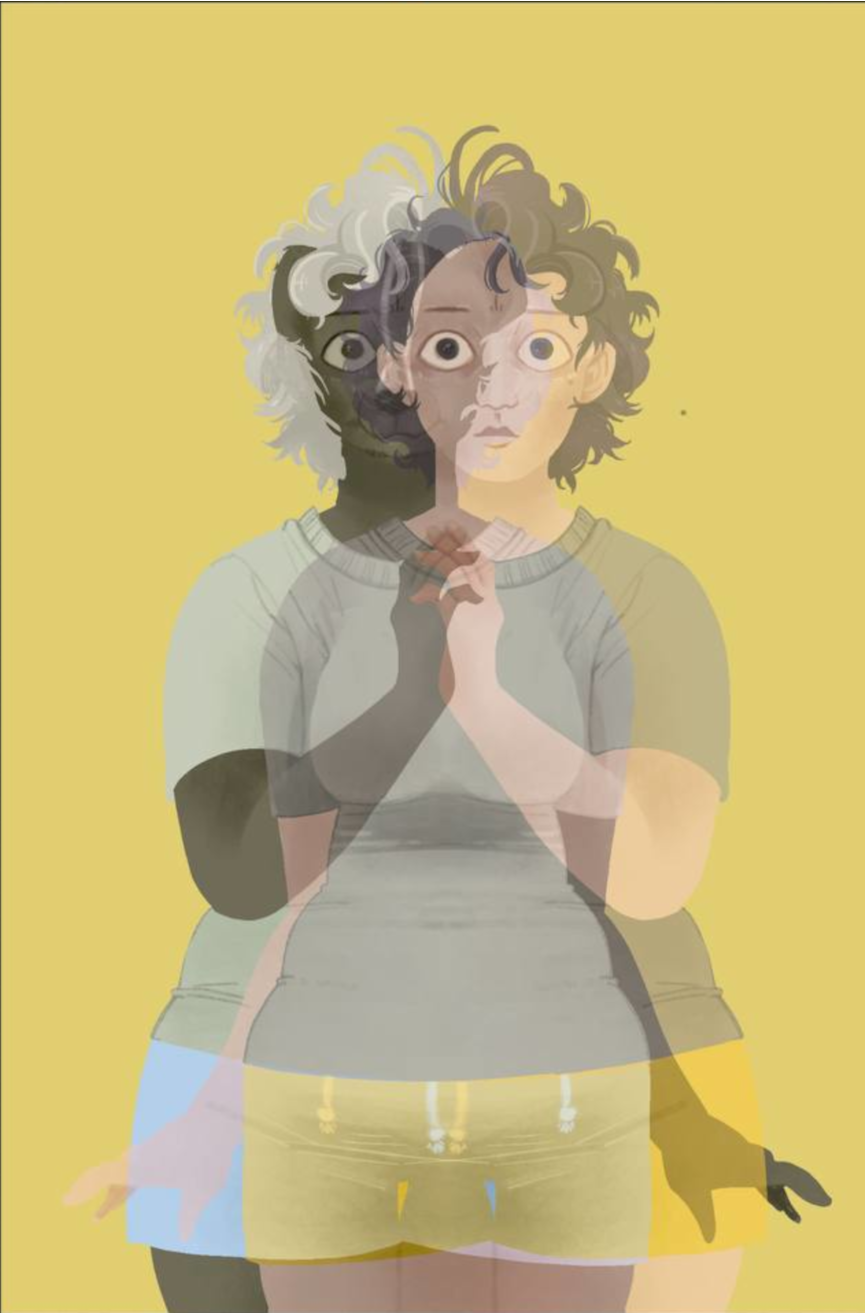
\includepdf[pages={1},offset=18pct 0]{assets/split}}

She rubbed at the back of her neck to ease the pain, then quickly pulled her hand away as though burnt.

Hand.

Paw.

Hand.

Paw.

Her body could not seem to make up its mind. Just as the fall seemed to explain the jolts of pain, the quaking in her body seemed to come from the way her form wobbled between states. Waves of skunk-fur/waves of human skin washed across her, gentle stripes moving through the base of human skin/through the base of skunk fur.

She screamed.

She screamed and the scream wobbled through different registers with an unnerving electric intensity that set her teeth on edge and made her fur bristle/made her skin crawl.

The scream did not echo.

What vasty nothing must produce such anechoic bliss! The silence hurt her ears, deafened her.

The scream cut short, she stumbled, ran, stumbled again, and kept running. Did not know where she ran. Did not care where she ran. Picked a direction and sprinted. Hoarse breathing echoed within her ears, for where else would it echo?

Hazardous glances back marked her distance by the shrinking of the lone bar, standing awkwardly amid flowers.

\emph{And I ran.} Words coursed absurdly through her head. Coursed and squirmed, slick to the touch. \emph{I ran so far away.} Words and music. Notes falling upon her from on high. Words welling up from somewhere deep within her gut.

She looked back, saw the bar dwindle, and when she turned around once more, skidded to a halt. For there was the bar again. Obstinately proving its presence through albedo and shadow and solidity. Looked behind her again and saw only empty field.

Screamed again.

Deafened again, fell silent.

Reached behind her for that cool draft against her neck, tried to pull back.

There was no draft.

There was no pulling back.

That pain, then: not the shock of falling from the stool, but the shock of sudden disconnection.

Fell to her knees and scrambled toward the bar on all fours, huddling against it and staring wide-eyed at the endless plain of dandelions. Heard her breath echo against the wood of the bar. Turned to face it and screamed deliberately, letting the subtle echo of acknowledgement, the presence of something solid, wash over her. Relished it. Screamed obscenities. Cursed the world. Cursed the powers that sent her to this place. Lost. Lost. Lost.

She could not control her thoughts. The world came at her too fast. An intrasaccadic smear of a world. A gesture at reality.

It was days/years/minutes until she was able to calm herself once more. The sun set/never set. The air temperature swung wildly to cold at night/was an unchanging warm that would not permit the passage of time.

Her mind wandered far.

Days passed.

Or not.

She plucked at a dandelion at some point, breathed in the fresh-baked scent of it. Let it fall to the ground.

She levered herself up onto the stool once more and cheerfully ordered herself a drink from no one. She clawed/scratched at the bar's stained and varnished surface, sobbing. Tears left tracks in fur/slid from her cheeks to the bar top.

And always her form shifted and danced. Her tail would sway into being and then it would never have been there. Her skin would sting and prickle from slamming her hand down against the bar and then that skin would be replaced by velvety pads.

She came to at some point/calmed down enough to think/let her breath slow enough that she was no longer sobbing.

Days passed.

Perhaps.

\emph{If this is a dream and I know it, do I not have control? Can I not make my reality for me?}

She breathed in to the count of four, held for the count of two, and then breathed herself out on a breath. There, beside her on the next stool, sat her human form/sat her skunk form. Her mind was split. Shared between the two. Neither could move without the other moving. Unison did not describe the perfection of the match.

But at least she was no longer out of focus.

\emph{Was this what the lost were going through?} She brushed her hand/paw through her hair/over her ears. \emph{Or perhaps it is merely a furry thing, primed as we are to have an internal representation so different from our external? Perhaps it is a me thing? Perhaps all are unique.}

``Oh AwDae,'' she moaned. ``Oh fox. How long have you been suffering?''

Days passed.

The sun rose and set with a frightening hum/utter tranquility.

She stood/she stood.

Poetry coursed through her, half remembered/perfectly memorized lines from productions long past. Lines from school, from work. ``Since then — 'tis centuries — and yet feels shorter than the day I first surmised the horse's heads were toward eternity —''

It \emph{had} been centuries for her, and yet each felt shorter than the crash to the ground from out of the perilous heights of the embodied world. \emph{Time feels so vast that were it not For an Eternity\ldots{}}

Time, which beat against the skies. Time, which hemmed her in. Time, which forced words from her mouth/from her muzzle in breathless haste/unwavering slowness. \emph{I fear me this Circumference Engross my Finity — To His exclusion who prepare By Process of Size For the Stupendous Vision Of his diameters —}

``Oh fox.''

She cried again/cried again. Sat on the ground again/sat on the ground again. Plucked a dandelion/plucked a dandelion. Again/again. Always twice over.

``Sasha!'' She spoke aloud.

``The fuck.'' Half question this time.

``Sasha, it's Debarre,'' she said. Then: ``What the fuck?''

``I'm so sorry. I came as fast as I could. Everything's a fucking mess.''

``How long has it been?'' she asked herself.

``About sixteen hours.''

``Hours?'' Hours? What meaning held time? She had lived her whole life — several such — on this tiny world.

``Yeah. I had to dump a chunk of my savings into a ticket to get here.''

She clawed at the ground in something between frustration and terror that a friend's voice was coming from her mouth/from her muzzle. ``And\ldots{}how are you\ldots{}''

``A mirror rig.'' The joyous tone of the words clashed against the tears still flowing freely. ``We figured it out. Carter figured it out, I mean. She and AwDae busted everything open. Figured out how to rescue the lost, figured out how everyone \emph{gets} lost in the first place.''

She stopped digging at the earth. ``AwDae is back?''

``Yes! And the clinic where Cicero is is trying to get him out as well!''

She had to turn toward the bar again to let the shouting echo. The silence was giving her a headache.

Or not. A neck-ache. Something was tearing at the back of the neck/through the fur of her scruff. An ache. A jolt of pain. A ripping. A tearing.

``I'm going to stop mirroring now. This is horrifying,'' she said to the wood of the bar. She did not know who said the last, Debarre or herself. Was there a difference?

And then, a hand on her shoulder. One of her shoulders. The sensation made her hair/fur stand on end. She turned around, and there was Debarre. Or so she guessed. The grey, default avatar. The figure frowned as he looked between the two of her. Looked at Michelle/looked at Sasha.

``I\ldots{}what? Sasha?''

She gritted her teeth/bared her teeth. ``I do not know either. What to we do now? How do we get out of this\ldots{}place?''

The shape that promised it was Debarre shrugged. ``Can you back out?''

She reached. Felt the draft. Smiled beatifically. She passed the field of dandelions. Passed the setting sun, or perhaps he passed her.

And breathed in the cool air of an implant clinic.

There, beside her, also sitting up from the recliner and pulling off his headband, was, she supposed, Debarre. Short. Soft. Thinning hair. Ecstatic grin.

``Sasha?'' The grin picked up an ironic twist. ``Or Michelle, I guess. You okay?''
